\documentclass[a4paper,kul]{kulakarticle} %options: kul or kulak (default)

\usepackage[utf8]{inputenc}
\usepackage[english]{babel}
\usepackage{graphicx}
\usepackage{subcaption}
\newlength{\twosubht}
\newsavebox{\twosubbox}
\graphicspath{{../Figures/}{../Matlab/}{/}}
\usepackage[outdir=./]{epstopdf}

\usepackage{tikz}
\usetikzlibrary{shapes,arrows}
\usepackage{verbatim}

\usepackage{amsmath}
\usepackage{siunitx}
\usepackage{amsthm}
\usepackage{amssymb}
\usepackage{gensymb}
\setcounter{MaxMatrixCols}{21}

\usepackage{etoolbox,refcount}
\usepackage{multicol}

\newcounter{countitems}
\newcounter{nextitemizecount}
\newcommand{\setupcountitems}{%
	\stepcounter{nextitemizecount}%
	\setcounter{countitems}{0}%
	\preto\item{\stepcounter{countitems}}%
}
\makeatletter
\newcommand{\computecountitems}{%
	\edef\@currentlabel{\number\c@countitems}%
	\label{countitems@\number\numexpr\value{nextitemizecount}-1\relax}%
}
\newcommand{\nextitemizecount}{%
	\getrefnumber{countitems@\number\c@nextitemizecount}%
}
\newcommand{\previtemizecount}{%
	\getrefnumber{countitems@\number\numexpr\value{nextitemizecount}-1\relax}%
}
\makeatother    
\newenvironment{AutoMultiColItemize}{%
	\ifnumcomp{\nextitemizecount}{>}{3}{\begin{multicols}{2}}{}%
		\setupcountitems\begin{itemize}}%
		{\end{itemize}%
		\unskip\computecountitems\ifnumcomp{\previtemizecount}{>}{3}{\end{multicols}}{}}

\usepackage{pdflscape}

\date{Academic year 2021 -- 2022}
\address{
  Faculty of Engineering Science \\
  Department of Mechanical Engineering \\
  Control theory \texttt{[H04X3a]}}
\title{Report Assignment 2: Velocity control of the cart}
\author{Matthias Derez, Toon Servaes}


\begin{document}

\maketitle

\tableofcontents
\listoffigures
\listoftables

\newpage
\section{Introduction}
In this report, two velocity controllers for a DC motor are designed, using frequency respons methods. The main criterion states that the velocity controller yields a zero steady-state error on a constant velocity reference. 
\section{Design of the controller}
\subsection{Type of controller}
\label{sec: typecontroller}
To satisfy the criterion of zero steady-state error, multiple controllers can be used. A PI, PID and feedforward controller can all yield a zero steady-state error. For the PI and PID controllers, this is caused by the integration part. The feedforward controller can be especially usefull for tracking and can eliminate errors induced by a changing reference value. However, as the controller must yield a zero steady-state error on a constant velocity reference and deal with errors caused by disturbances, the feedforward controller will not be used. Since a large bandwidth yields a fast responding system, a high bandwidth seems advantageous. If the bandwidth is too high though, the high frequency noise has more influence. A trade-off between the two has to be made. Additionally, the overshoot $M_p$ must be kept sufficiently low. High peaks in the transient respons have to be avoided, as the Arduino can only deliver voltages in a range of $[-12V, 12V]$. If high peaks are present in the respons, it is possible the controller wants to send out voltages outside this range. This is ofcourse impossible, which makes the cart unable to follow the correct respons imposed by the controller. %Generally the sampling frequency has to be at least 10-20 times larger than bandwidth (\underline{REFERENTIE C8 S82}). In this report, the bandwidth will be approximated by the crossover frequency $\omega_c$.%
Because of the aforementioned reasons and because of simplicity the PI controller is chosen.
\subsection{Design parameters}
To properly execute the design, some design parameters must be determined. The parameters that can be chosen free are the phase margin PM and the extra margin $d\phi$ to compensate for the phase lag of the PI controller. Using these, the new cross over frequency $\omega_c$, the integration time $T_i$, the gain K and the gain margin GM of the controller can be calculated. 
%Firstly, we write down the used values and equations, later on additional information will be given on why these values are chosen and the relations between the variables.% 



\subsubsection{Phase margin}
The design value of the PM can vary from 40\degree to 50\degree. From chapter 7 of the course notes "Control Theory- Handouts" \cite{slidescontroltheory}, we know that by increasing the PM, the dampingratio $\zeta$ and $T_i$ will increase. The peak value in the closed loop step response $M_p$ and the new cross over frequency $\omega_c$ will decrease. The increase in $\zeta$ causes the respons of the signal to be slower, but have less oscillations. Since the value of $\zeta$ is still below the value of critical damping of $\zeta = 0.7$, the increase is in general advantageous for the transient respons. The decrease of $\omega_c$ %helps to keep the cross over frequency 10-20 times lower than the sampling frequency and%
 reduces the influence of high frequency noise. However, $\omega_c \gg \frac{1}{T_i}$ is necessary to lower the influence of the phase lag introduced by the PI controller. Luckily by increasing the PM, $\frac{1}{T_i}$ decreases (see Equation \ref{eq: Ti}) and thus the fact that $\omega_c$ reduces, is partly compensated by the decrease in $\frac{1}{T_i}$. The decrease in overshoot $M_p$ improves the transient respons. By processing the data in \texttt{Matlab}, it becomes clear that by increasing the PM, the GM increases and the transient errors decreases. For these reasons, the PM is chosen to be equal to 50\degree. 

\subsubsection{Extra margin to compensate for the phase lag}
	As the PI controller has a negative phase, an extra margin $d\phi$ on the PM has to be included to calculate the new cross over frequency $\omega_c$. The chosen margin can vary from 10\degree to 15\degree. By choosing a higher value, the GM increases and the gain decreases, which helps to reduce resonance. By using different values and calculating the stepresponse on the closed loop system in \texttt{Matlab}, it is clear the transient errors decreases when the extra margin is increased. $d\phi = 15\degree$ is chosen. 

\subsubsection{General design procedure}
\label{sec:designprocedure}
Now the PM and the extra margin on the PM have been chosen, the frequency where the uncompensated open loop system has a phase $\phi = -180\degree + PM + d\phi$ can be determined. This is the new cross over frequency $\omega_c$. Using this result, $T_i$ can be calculated using Equation \ref{eq: Ti}. 

\begin{equation}
	\label{eq: Ti}
	T_i = \frac{\tan(90\degree - d\phi)}{\omega_c}
\end{equation} 
The transfer function of the PI controller can be written as:
\begin{equation}
	\label{eq: TF PI}
	D(s) = \frac{K}{s}(s+\frac{1}{T_i})
\end{equation}
The gain K can be determined, stating that the gain of the compensated system at $\omega_c$ indeed equals 1:
\begin{equation}
	|G(j\omega_c)D(j\omega_c)| = 1
\end{equation}
The gain margin is a measure for stability and reduces resonance. The design value is $GM \approx 2 \approx 6 dB$. The values obtained from these calculations can be found in Table \ref{tab:values}. 

\begin{table}[htp!]
	
	\centering
	
	\begin{tabular}{|l|l|l|}
		\hline
		Parameter                & Value motor A & Value motor B                       \\ \hline
		GM                       & 1.6733 &        1.6241                \\
		PM                       & 49.2211\degree & 49.2477\degree \\
		$\omega_c$ & 60.9960 rad/s              &  62.9272 rad/s\\
		$T_i $                    & 0.0612 s    &     0.0592s           \\
		$\frac{1}{T_i}$                    & $16.3473 s^{-1}$  &  $16.8808s^{-1}$                  \\
		$d\phi$             & 15\degree    & 15\degree \\
		gain K 	 		& 1.0712  & 1.0225 \\  \hline
	\end{tabular}
	\caption{Design parameters and their calculated values using general design method}
	\label{tab:values}
\end{table}
%As can be seen in Table \ref{tab:values}, however the difference is quite small and the system shows no sign of instabilities, the value is acceptable. $\frac{1}{T_i}$ is not that much smaller than $\omega_c$, but the influence of the extra phase lag on the other parameters is acceptable. In Figure \ref{fig:bodeplotopenloop} the bodeplots of the different open loop systems are shown and in Figure \ref{fig:bodeplotcl} the bodeplot of the closed loop system is shown. %
Next to the values in Table \ref{tab:values}, the open loop (= serial connection of controller and model) and closed loop bodediagrams are shown in Figure \ref{fig:bodeplotopenloopmethod1} and Figure \ref{fig:bodeplotclmethod1} respectively. The closed loop step responses are shown in Figure \ref{fig:stepresponseclmethod1}. Several factor show this controller is not optimal. First of all the GM does not meet the required value of 2. This means the system can become unstable or contain resonance. The latter is reflected in the resonance peak in the bodeplot of the closed loop system in Figure \ref{fig:bodeplotclmethod1}. In Figure \ref{fig:stepresponseclmethod1}, a high overshoot value $M_p$ can be observed. This can cause troubles, as discussed earlier in Section \ref{sec: typecontroller}. 





\begin{figure*}[htp!]
	\centering
	\begin{subfigure}[b]{0.49\textwidth}
		\centering
		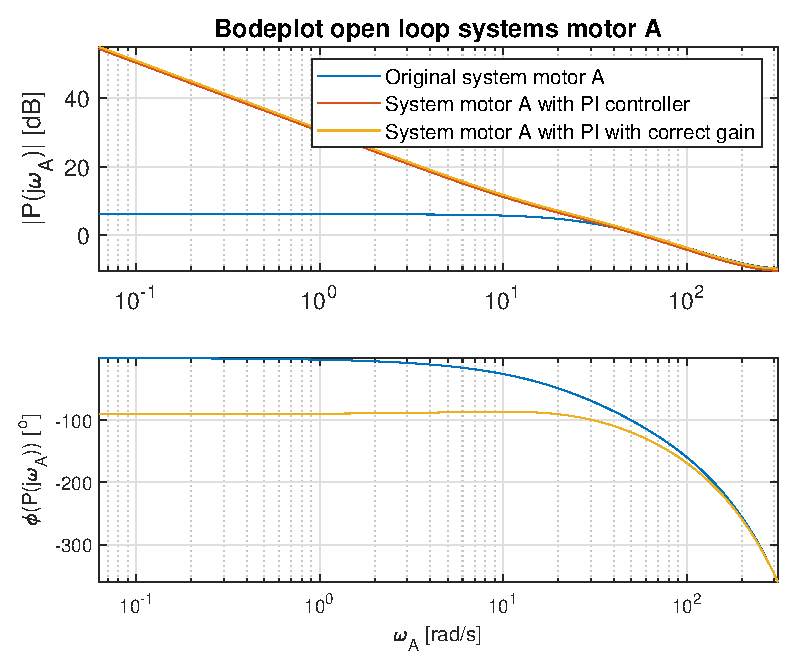
\includegraphics[width=\linewidth]{bodeplotA_openloop_method1.eps}
		
	\end{subfigure}
	\hfill
	\begin{subfigure}[b]{0.49\textwidth}  
		\centering
		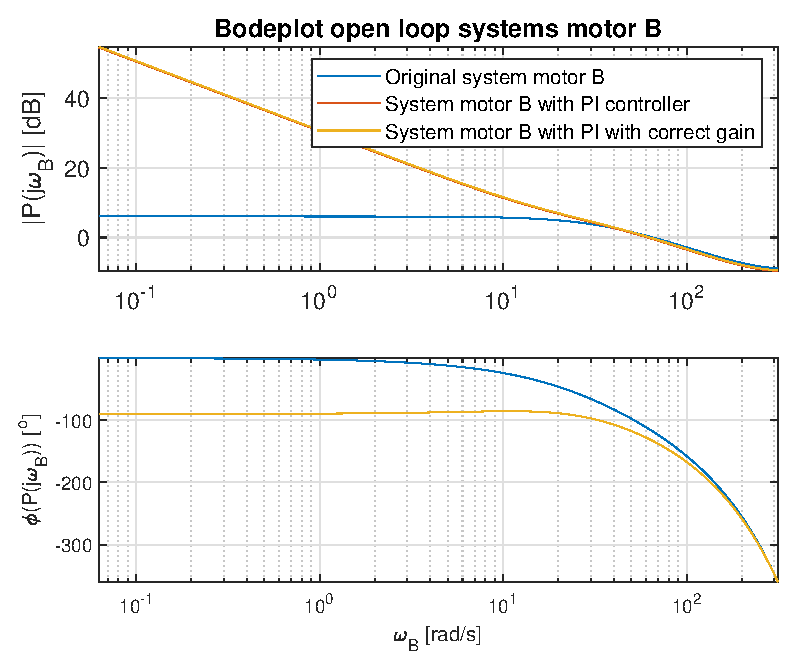
\includegraphics[width=\linewidth]{bodeplotB_openloop_method1.eps}
		
	\end{subfigure}
	\caption{Bodeplot of the different open loop systems using the general design method}
	\label{fig:bodeplotopenloopmethod1}
\end{figure*}

\begin{figure*}[htp!]
	\centering
	\begin{subfigure}[b]{0.49\textwidth}
		\centering
		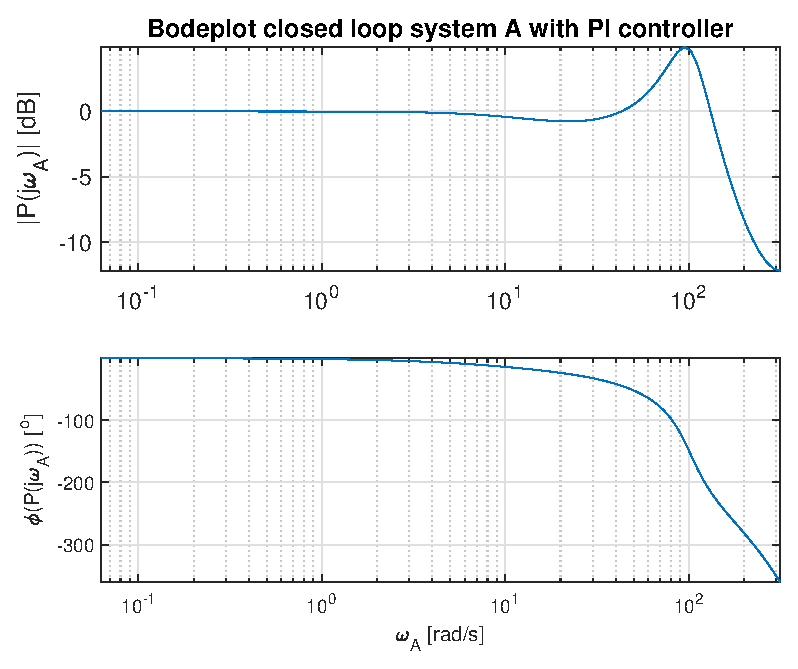
\includegraphics[width=\linewidth]{bodeplotA_cl_method1.eps}
		
	\end{subfigure}
	\hfill
	\begin{subfigure}[b]{0.49\textwidth}  
		\centering
		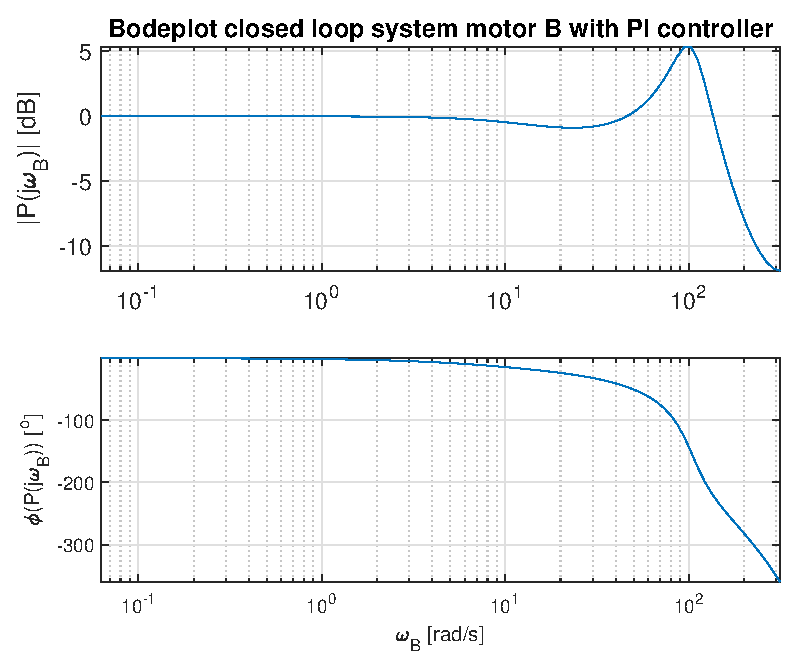
\includegraphics[width=\linewidth]{bodeplotB_cl_method1.eps}
		
	\end{subfigure}
	\caption{Bodeplot of the closed loop system with PI controller using the general design method}
	\label{fig:bodeplotclmethod1}
\end{figure*}

\begin{figure*}[htp!]
	\centering
	\begin{subfigure}[b]{0.485\textwidth}
		\centering
		\includegraphics[width=\linewidth]{stepresponsA_cl_method1.eps}
		
	\end{subfigure}
	\hfill
	\begin{subfigure}[b]{0.5\textwidth}  
		\centering
		\includegraphics[width=\linewidth]{stepresponsB_cl_method1.eps}
		
	\end{subfigure}
	\caption{Step response of the closed loop system with PI controller using the general design method}
	\label{fig:stepresponseclmethod1}
\end{figure*}

\newpage
\subsubsection{Improvement of the controller}
In section \ref{sec:designprocedure}, it became clear the general design procedure does not provide an acceptable controller. To improve the controller, two methods were considered. First of all, the gain could be lowered to increase the GM and PM, while keeping the same $T_i$. Secondly the desired GM given in the design could be increased. Comparison of the two methods for several values in \texttt{Matlab} showed that the first method (decreasing gain K) produced the best system parameters, for example higher GM for the same PM, lower overshoot and a far better transient respons to a step input in general. By a method of trial and error, following values for the gain were selected: 
\begin{equation}
	\begin{split}
	Motor A: K_a &= 0.8\\
	Motor B: K_b &= 0.775
	\end{split}
\end{equation}
These gains yield the values given in Table \ref{tab:valuesmethod2}. 

\begin{table}[htp!]
	
	\centering
	
	\begin{tabular}{|l|l|l|}
		\hline
		Parameter                & Values motor A & Values motor B                       \\ \hline
		GM                       & 2.2406 &        2.1427                \\
		PM                       & 68.5401\degree & 69.1969\degree \\
		$\omega_c$ & 42.1655 rad/s              &  43.65972 rad/s\\
		$T_i $                    & 0.0612 s    &     0.0592 s           \\
		$\frac{1}{T_i}$                    & $\SI{16.3473}{s^{-1}} $  &  $\SI{16.8808}{s^{-1}} $                 \\
		$d\phi$             & 15\degree    & 15\degree \\
		gain K 	 		& 0.8000  & 0.7750 \\ 
		Closed loop bandwidth & 121.5664 rad/s & 128.2576 rad/s \\ \hline
	\end{tabular}
	\caption{Design parameters and their calculated values using the improved design method}
	\label{tab:valuesmethod2}
\end{table}
In Figure \ref{fig:bodeplotopenloopmethod2} we see the bodeplot of the open loop system (= serial connection of the controller and the model). The improved values for the GM and PM from Table \ref{tab:valuesmethod2} are shown in this figure. Apart from that, from Figure \ref{fig:bodeplotopenloopmethod2} it becomes clear the DC-value of the open loop system goes to infinity. This proves the steady-state error of the closed loop goes to zero. In Figure \ref{fig:bodeplotopenloopmethod2multiple}, the different open loop systems are shown and in Figure \ref{fig:bodeplotclmethod2}, the bodeplots of the closed loop systems are displayed. Comparing Figures \ref{fig:bodeplotclmethod1} and \ref{fig:bodeplotclmethod2}, the resonance peak is clearly suppressed using the improved controller. In addition, the overshoot is lowered, as can be seen in Figure \ref{fig:stepresponseclmethod2}. The only disadvantage of this method is the decrease in open loop bandwidth. 
\begin{figure*}[htp!]
	\centering
	\begin{subfigure}[b]{0.49\textwidth}
		\centering
		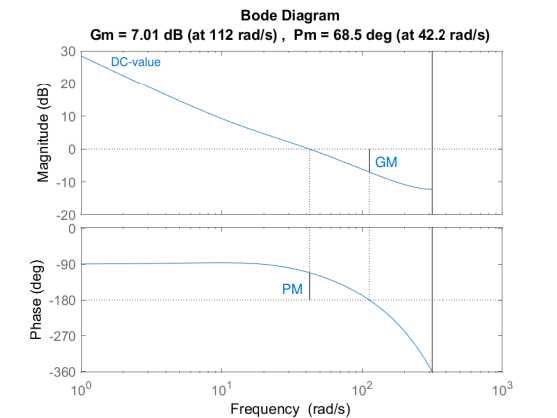
\includegraphics[width=\linewidth]{bodeplot_contr_sysA_openloop_method2.png}
		\caption{Motor A}
	\end{subfigure}
	\hfill
	\begin{subfigure}[b]{0.49\textwidth}  
		\centering
		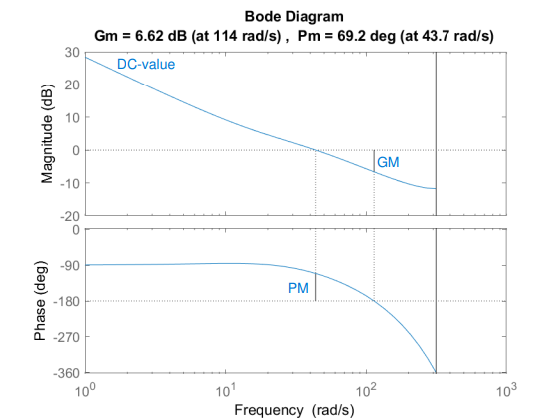
\includegraphics[width=\linewidth]{bodeplot_contr_sysB_openloop_method2.png}
		\caption{Motor B}
	\end{subfigure}
	\caption{Bodeplot of the open loop systems using the improved controller}
	\label{fig:bodeplotopenloopmethod2}
\end{figure*}
\begin{figure*}[htp!]
	\centering
	\begin{subfigure}[b]{0.49\textwidth}
		\centering
		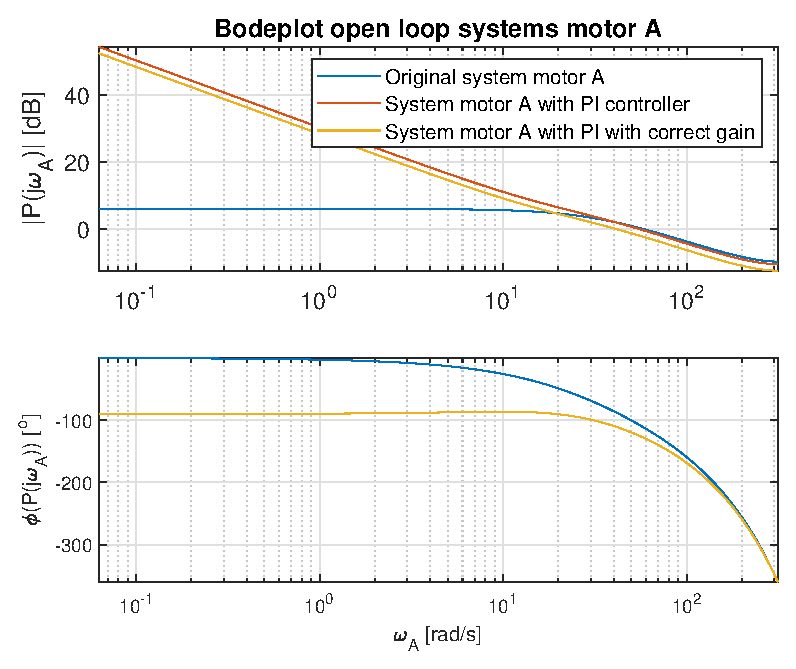
\includegraphics[width=\linewidth]{bodeplotA_openloop_method2.eps}
		
	\end{subfigure}
	\hfill
	\begin{subfigure}[b]{0.49\textwidth}  
		\centering
		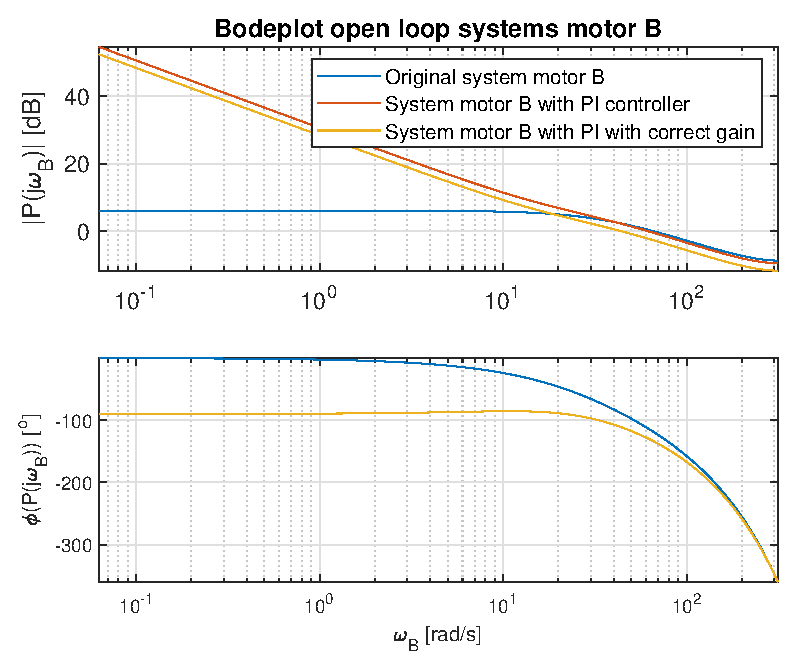
\includegraphics[width=\linewidth]{bodeplotB_openloop_method2.eps}
		
	\end{subfigure}
	\caption{Bodeplot of the different open loop systems using the improved controller}
	\label{fig:bodeplotopenloopmethod2multiple}
\end{figure*}

\begin{figure*}[htp!]
	\centering
	\begin{subfigure}[b]{0.49\textwidth}
		\centering
		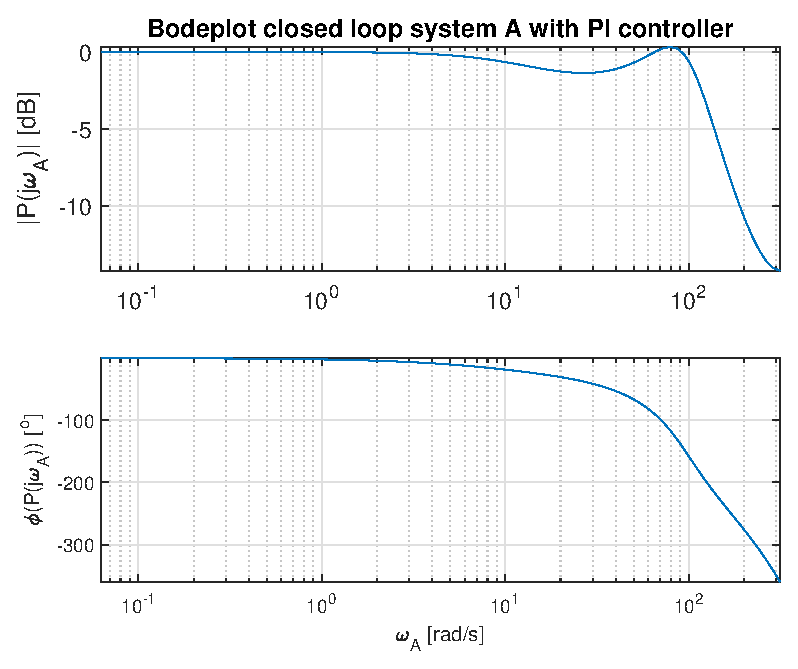
\includegraphics[width=\linewidth]{bodeplotA_cl_method2.eps}
		
	\end{subfigure}
	\hfill
	\begin{subfigure}[b]{0.49\textwidth}  
		\centering
		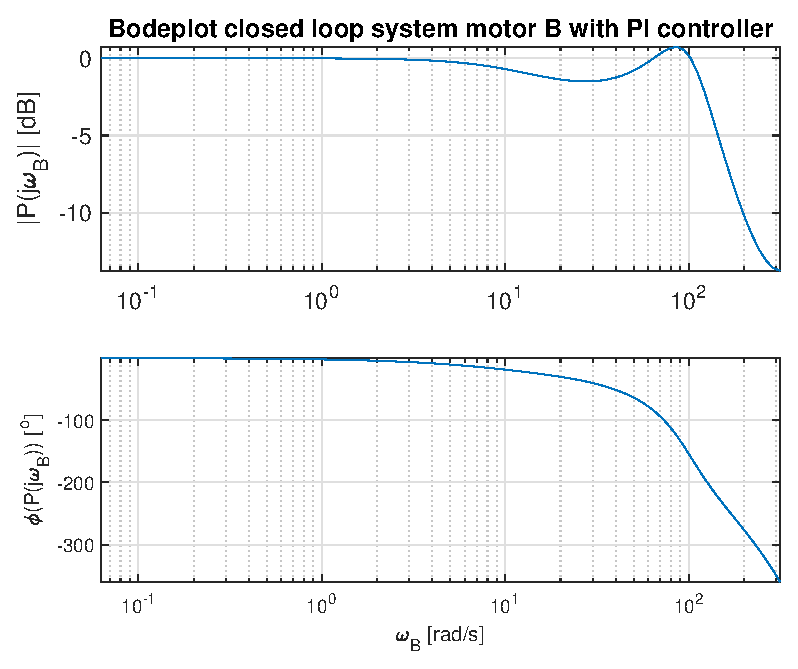
\includegraphics[width=\linewidth]{bodeplotB_cl_method2.eps}
		
	\end{subfigure}
	\caption{Bodeplot of the closed loop system with PI controller using the improved controller}
	\label{fig:bodeplotclmethod2}
\end{figure*}

\begin{figure*}[htp!]
	\centering
	\begin{subfigure}[b]{0.49\textwidth}
		\centering
		\includegraphics[width=\linewidth]{stepresponsA_cl_method2.eps}
		
	\end{subfigure}
	\hfill
	\begin{subfigure}[b]{0.49\textwidth}  
		\centering
		\includegraphics[width=\linewidth]{stepresponsB_cl_method2.eps}
		
	\end{subfigure}
	\caption{Step response of the closed loop system with PI controller using the improved controller}
	\label{fig:stepresponseclmethod2}
\end{figure*}
\newpage
\subsection{Limitations on the bandwidth}
The Nyquist theorem states that a signal can be constructed without aliasing if the sampling frequency $f_s$ is at least two times higher than the highest frequency in the system. This means the theoretical limitation on the closed-loop bandwidth is $\frac{f_s}{2}$, which equals $\SI{50}{Hz}$ in our case as the sampling frequency equals $\SI{100}{Hz}$. In practice, increasing the bandwith to the theorethical limit can pose problems, since the PM decreases with increasing bandwidth. However, the PM has a great influence on stability of the system and other parameters such as the overshoot and damping ratio. This means a minimal PM is often required, since the system has to be stable or the overshoot can't be too large because of the finite voltage range of the controller. For this reason the practical limit for the closed loop bandwidth can be lower than the theorethical limit. 

\section{Validation of the controller}
In this section the controller designed in the previous sections is validated experimentally. To do this, the controller is implemented in Arduino and a step input of $\SI{6}{rad/s}$ is applied for the reference velocity. In Figure \ref{fig:comparisonstepresponse} the different responses are shown, with a more zoomed in view on the transient response in Figure \ref{fig:comparisonstepresponsezoom}. The tracking error of the step reference is shown in Figure \ref{fig:trackingerrorstepresponse} with a close-up in Figure \ref{fig:trackingerrorstepresponsezoom}. From the aforementioned figures, it is clear the steady-state error of the simulated response goes to zero. For steady-state value of the measured response, there are still some deviations from the step reference. These are caused by measurement noise. Since the deviatons occur around the step reference value, the conclusion can be made the measuered steady-state error also equals zero, excluding measurement noise. Figure \ref{fig:trackingerrorstepresponsezoom} shows that the tracking error is maximal in the beginning for two time delays and equal to the value of the step reference. This is caused by the 2 timedelays between the input voltages and output wheel velocity of the system, which is discussed in Assignment 1. 

\begin{figure*}[htp!]
	\centering
	\begin{subfigure}[b]{0.49\textwidth}
		\centering
		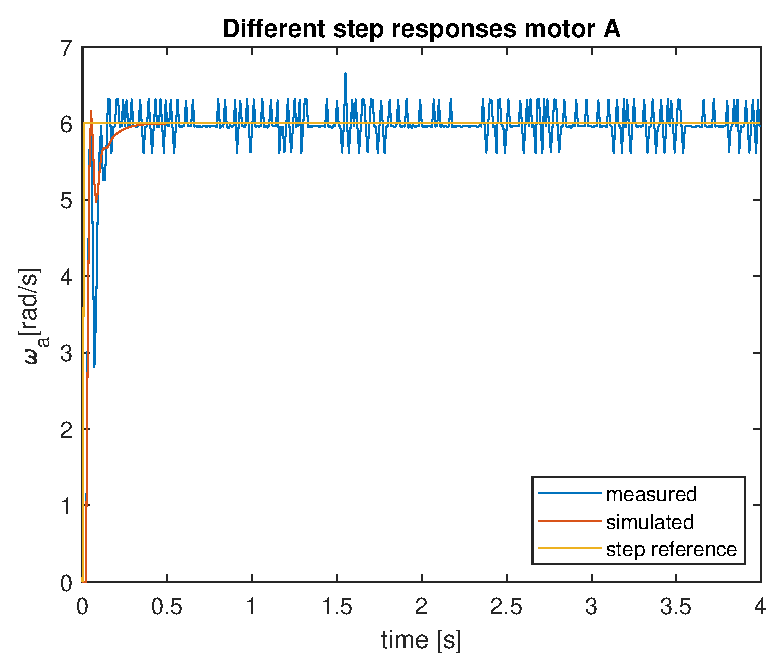
\includegraphics[width=\linewidth]{comparison_stepresponseA.eps}
		
	\end{subfigure}
	\hfill
	\begin{subfigure}[b]{0.49\textwidth}  
		\centering
		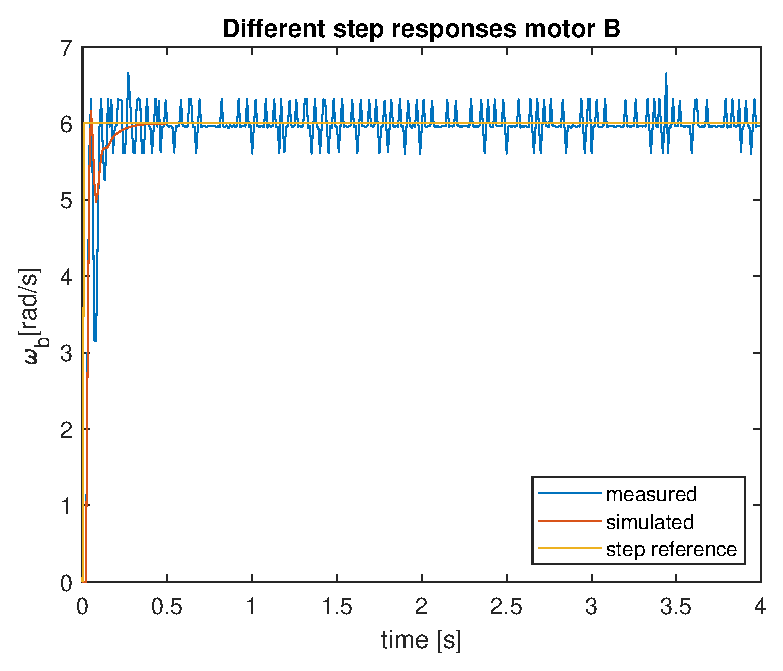
\includegraphics[width=\linewidth]{comparison_stepresponseB.eps}
		
	\end{subfigure}
	\caption{Measured and simulated responses of the closed loop system to a step input of $\SI{6}{rad/s}$ as reference velocity}
	\label{fig:comparisonstepresponse}
\end{figure*}

\begin{figure*}[htp!]
	\centering
	\begin{subfigure}[b]{0.49\textwidth}
		\centering
		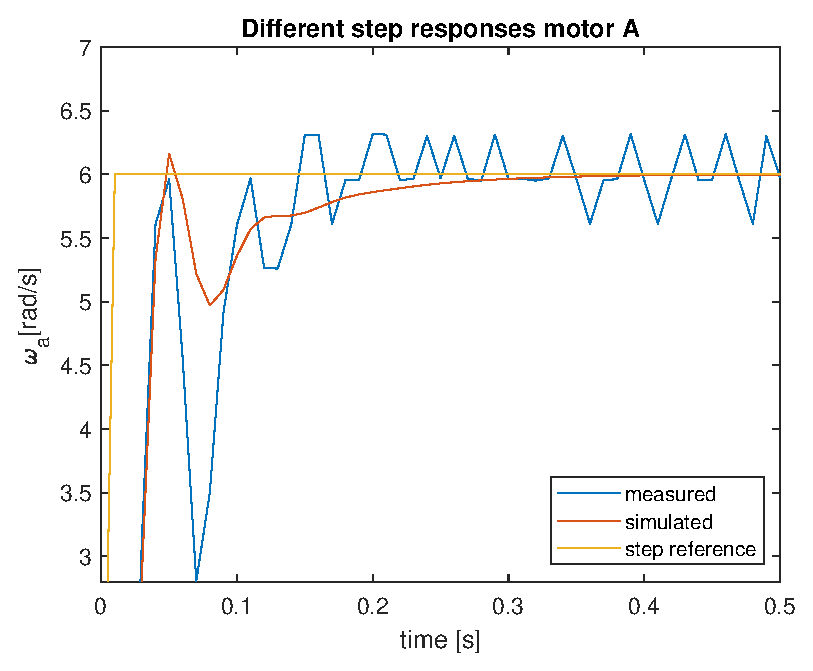
\includegraphics[width=\linewidth]{comparison_stepresponseA_zoom.eps}
		
	\end{subfigure}
	\hfill
	\begin{subfigure}[b]{0.49\textwidth}  
		\centering
		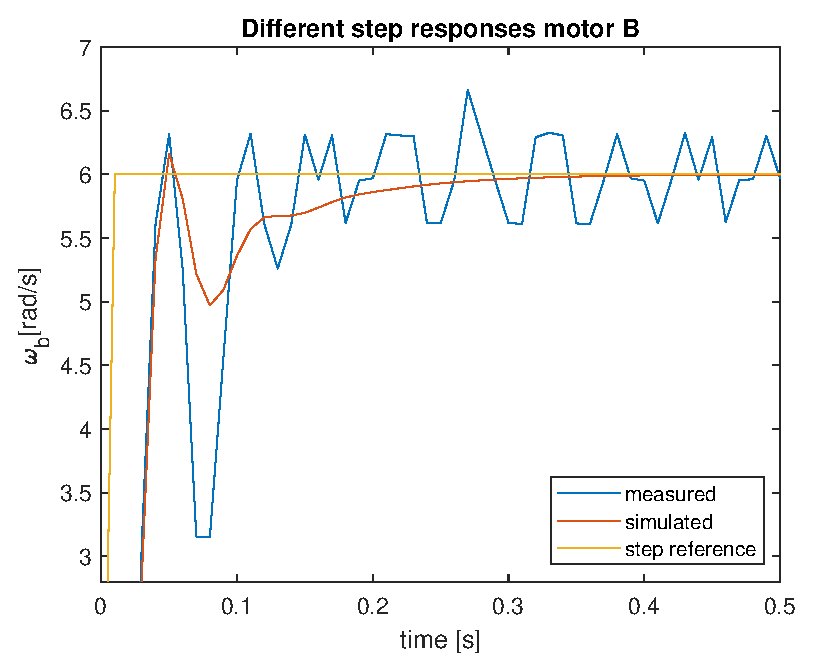
\includegraphics[width=\linewidth]{comparison_stepresponseB_zoom.eps}
		
	\end{subfigure}
	\caption{Close-up of the measured and simulated responses of the closed loop system to a step input of $\SI{6}{rad/s}$ as reference velocity}
	\label{fig:comparisonstepresponsezoom}
\end{figure*}

\begin{figure*}[htp!]
	\centering
	\begin{subfigure}[b]{0.49\textwidth}
		\centering
		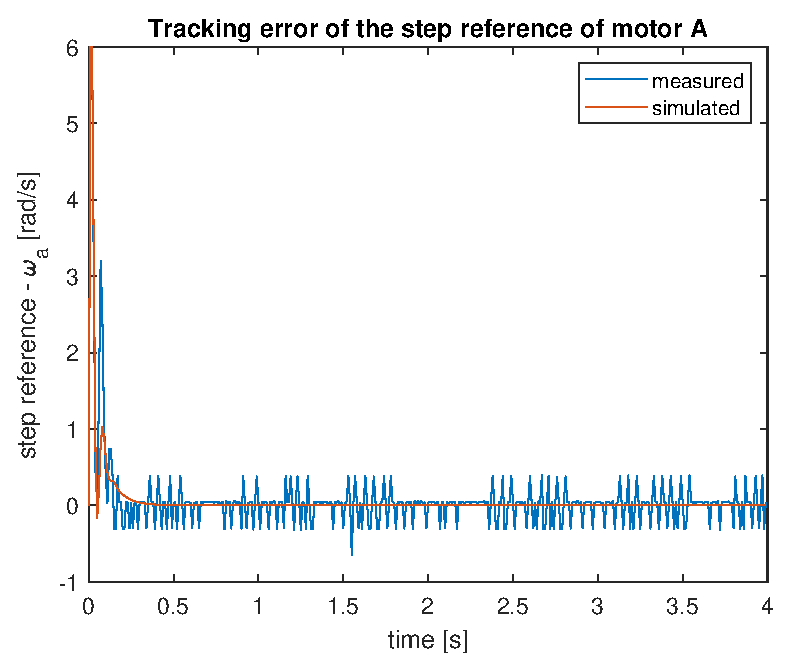
\includegraphics[width=\linewidth]{trackingerror_stepresponseA.eps}
		
	\end{subfigure}
	\hfill
	\begin{subfigure}[b]{0.49\textwidth}  
		\centering
		\includegraphics[width=\linewidth]{trackingerror_stepresponseB.eps}
		
	\end{subfigure}
	\caption{Measured and simulated tracking error of the closed loop system to a step input of $\SI{6}{rad/s}$ as reference velocity}
	\label{fig:trackingerrorstepresponse}
\end{figure*}

\begin{figure*}[htp!]
	\centering
	\begin{subfigure}[b]{0.49\textwidth}
		\centering
		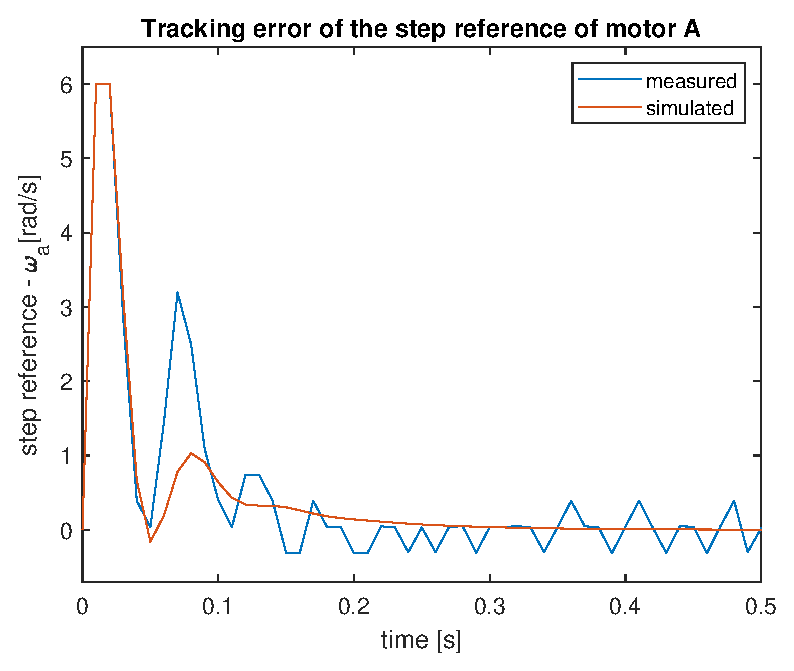
\includegraphics[width=\linewidth]{trackingerror_stepresponseA_zoom.eps}
		
	\end{subfigure}
	\hfill
	\begin{subfigure}[b]{0.49\textwidth}  
		\centering
		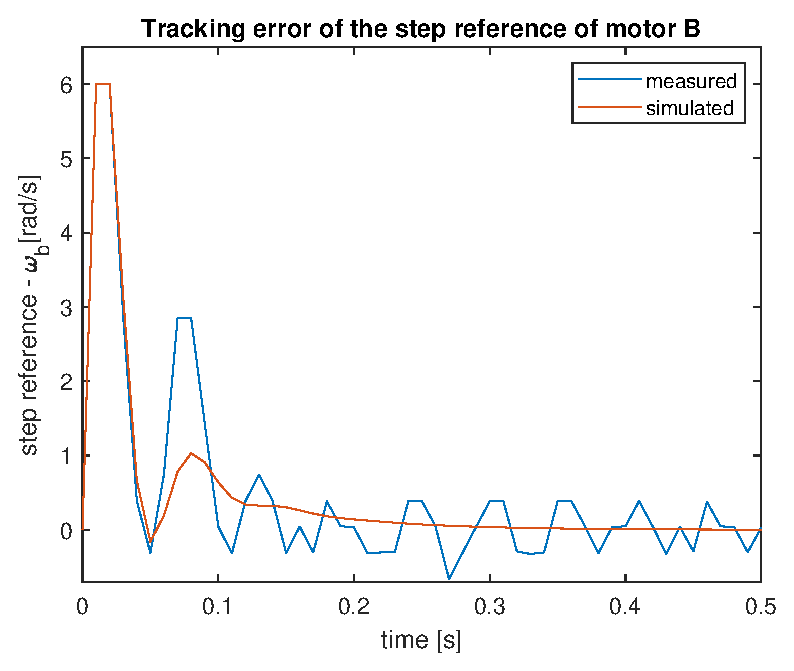
\includegraphics[width=\linewidth]{trackingerror_stepresponseB_zoom.eps}
		
	\end{subfigure}
	\caption{Close-up of the measured and simulated tracking error of the closed loop system to a step input of $\SI{6}{rad/s}$ as reference velocity}
	\label{fig:trackingerrorstepresponsezoom}
\end{figure*}

Figure \ref{fig:voltagestepresponse} shows the measured and simulated voltages (control signals) for the step input reference. We know that as the time increases, the error of the simulated model response goes to zero. This can be seen in Figure \ref{fig:voltagestepresponse}, as the simulated voltages reach a constant value. There are still variations in the measured voltages, these do not converge to a constant value due to the fact that the error on the measured response does not go to zero exactly.
\begin{figure*}[htp!]
	\centering
	\begin{subfigure}[b]{0.49\textwidth}
		\centering
		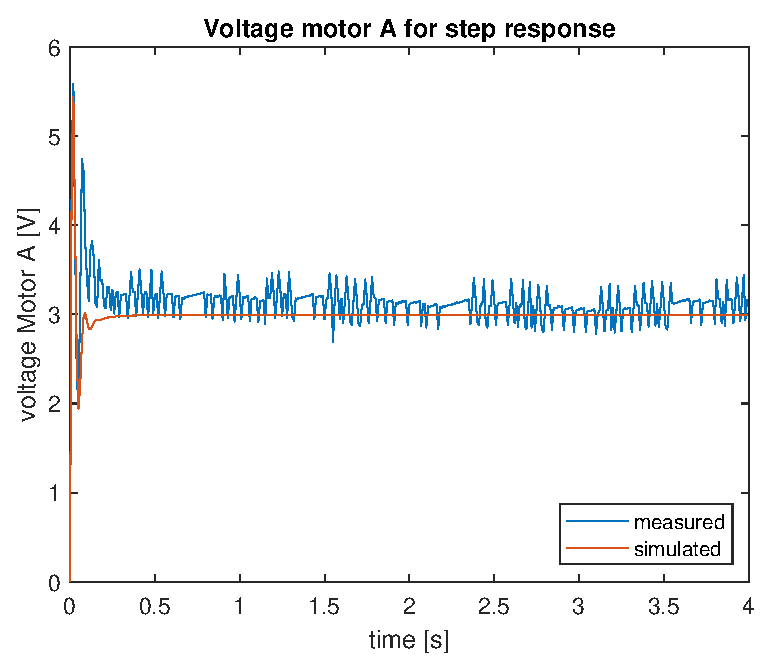
\includegraphics[width=\linewidth]{comparison_voltage_stepresponseA.eps}
		
	\end{subfigure}
	\hfill
	\begin{subfigure}[b]{0.49\textwidth}  
		\centering
		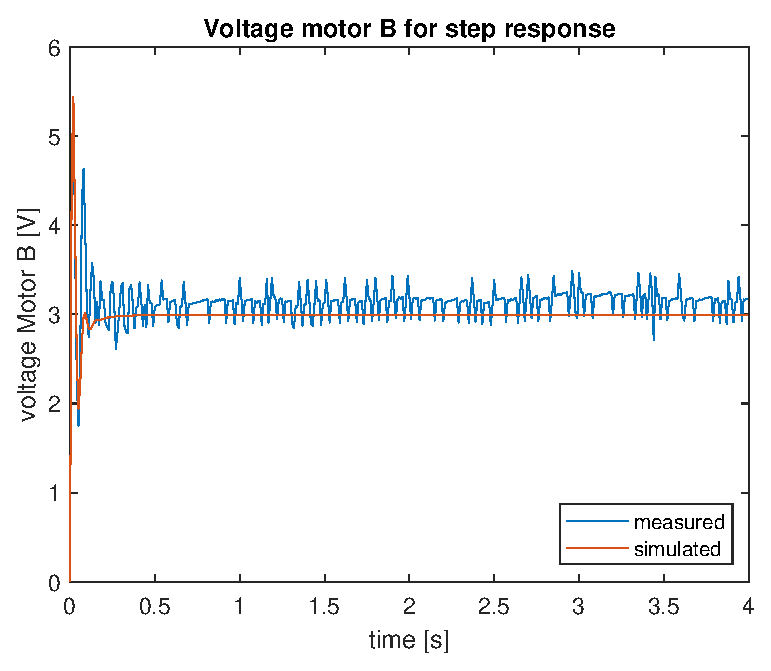
\includegraphics[width=\linewidth]{comparison_voltage_stepresponseB.eps}
		
	\end{subfigure}
	\caption{Measured and simulated voltages for a step reference input}
	\label{fig:voltagestepresponse}
\end{figure*}
\newpage
\subsection{Force disturbance}
To apply a constant force disturbance, the cart is placed on a slope instead of a horizontal surface. When the cart drives uphill, gravity creates a constant force opposite to the driving direction. The magnitude of the force is given by Equation \ref{eq:Fz}, where m is the mass of the cart and $\alpha$ is the slope angle (= $3.518\degree$ in our case). 
\begin{equation}
	\label{eq:Fz}
	F = m\cdot g\cdot \sin(\alpha)
\end{equation}
The disturbance enters the loop after the system, but is included within the feedback loop. This is shown in the block diagram in Figure \ref{fig: blockdiagram}.
\begin{figure}[htp!]
	\centering
	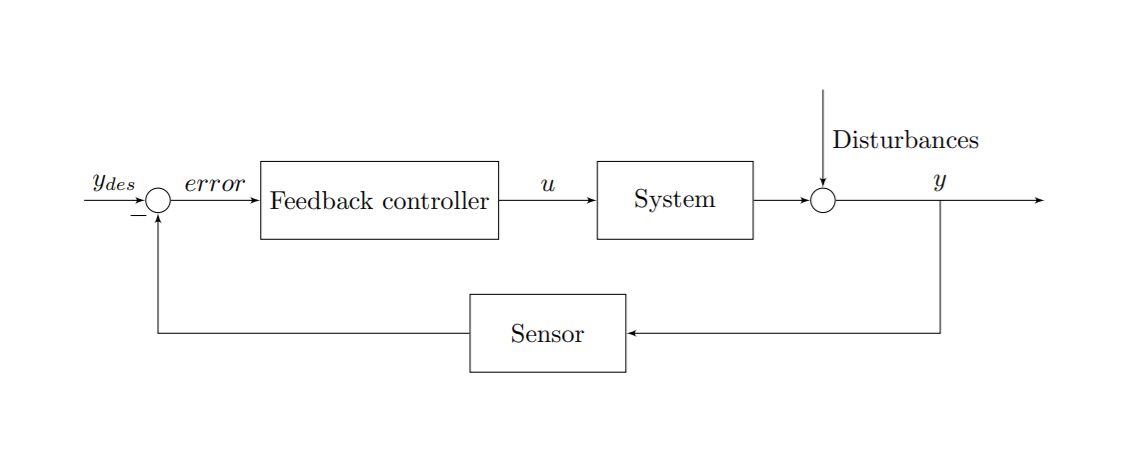
\includegraphics[width=\linewidth]{blockdiagram.png}
	\caption{Block diagram of control configuration with force disturbance \cite{tikz}}
	\label{fig: blockdiagram}
\end{figure}

In Figure \ref{fig:comparisonstepresponseFD} the measured and simulated responses to the step input as reference velocity are shown, while Figure \ref{fig:trackingerrorstepresponseFD} shows the tracking errors. These figures clearly indicate that the output velocity still follows the reference velocity with a steady-state error equal to zero. This can be explained looking at the block diagram in Figure \ref{fig: blockdiagram}. As the force disturbance is included within the feedback loop, the controller can take into account the error caused by the constant force disturbance and thus ensure the steady-state error to go to zero. Figure \ref{fig:voltagestepresponseFD} shows the measured control signal is higher than the simulated one. This makes sense, as a higher voltage is needed to overcome the force disturbance while maintaining the same speed. 

\begin{figure*}[htp!]
	\centering
	\begin{subfigure}[b]{0.49\textwidth}
		\centering
		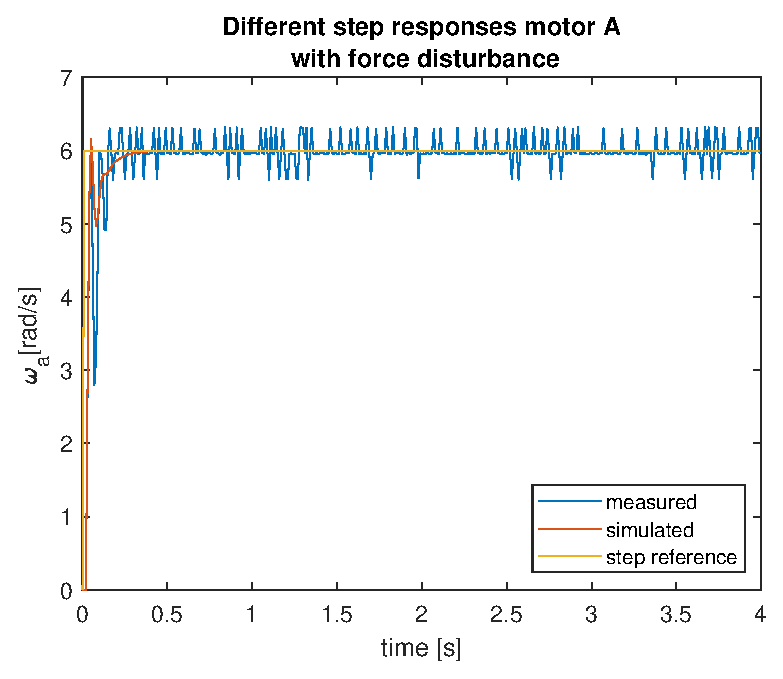
\includegraphics[width=\linewidth]{comparison_stepresponseA_FD.eps}
		
	\end{subfigure}
	\hfill
	\begin{subfigure}[b]{0.49\textwidth}  
		\centering
		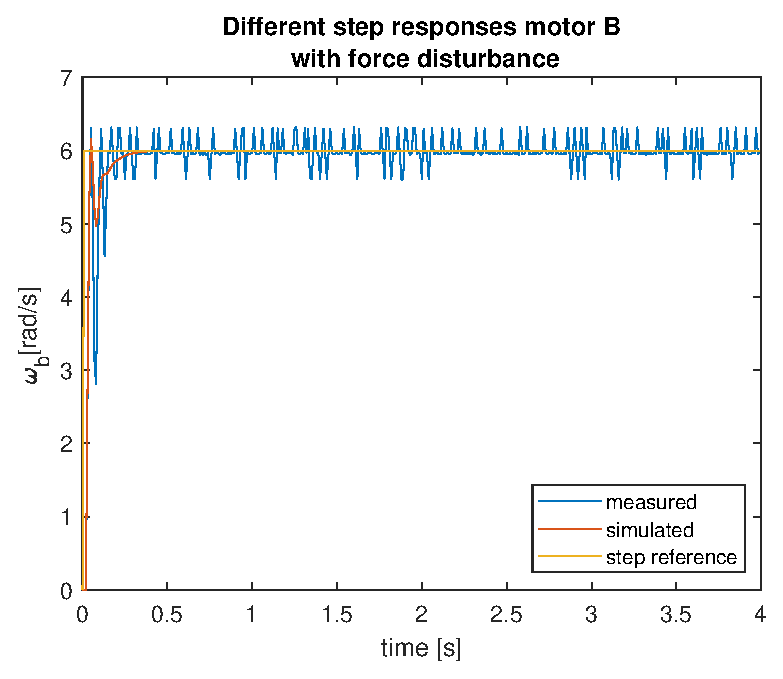
\includegraphics[width=\linewidth]{comparison_stepresponseB_FD.eps}
		
	\end{subfigure}
	\caption{Measured and simulated responses of the closed loop system to a step input of $\SI{6}{rad/s}$ as reference velocity with a constant force disturbance}
	\label{fig:comparisonstepresponseFD}
\end{figure*}

\begin{figure*}[htp!]
	\centering
	\begin{subfigure}[b]{0.49\textwidth}
		\centering
		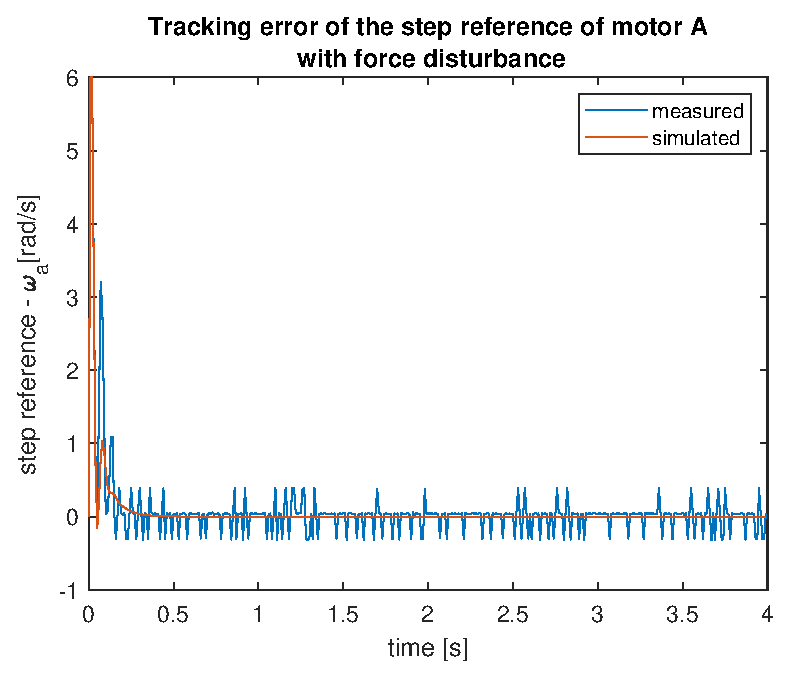
\includegraphics[width=\linewidth]{trackingerror_stepresponseA_FD.eps}
		
	\end{subfigure}
	\hfill
	\begin{subfigure}[b]{0.49\textwidth}  
		\centering
		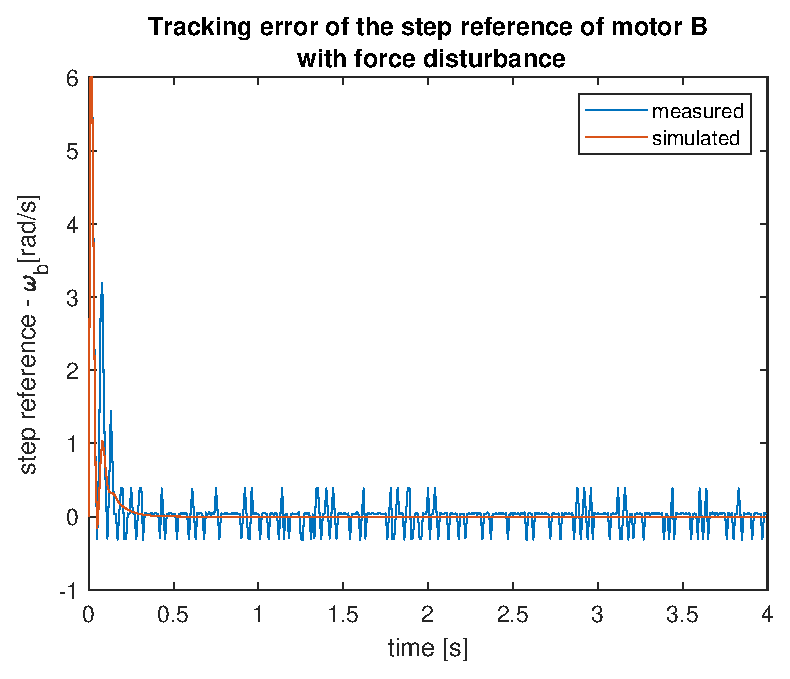
\includegraphics[width=\linewidth]{trackingerror_stepresponseB_FD.eps}
		
	\end{subfigure}
	\caption{Measured and simulated tracking error of the closed loop system to a step input of $\SI{6}{rad/s}$ as reference velocity with a constant force disturbance}
	\label{fig:trackingerrorstepresponseFD}
\end{figure*}

\begin{figure*}[htp!]
	\centering
	\begin{subfigure}[b]{0.49\textwidth}
		\centering
		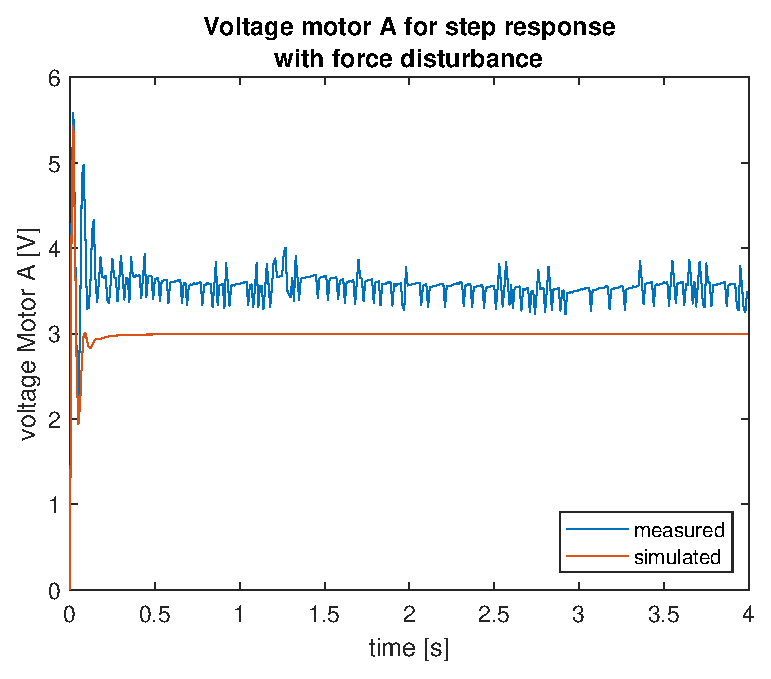
\includegraphics[width=\linewidth]{comparison_voltage_stepresponseA_FD.eps}
		
	\end{subfigure}
	\hfill
	\begin{subfigure}[b]{0.49\textwidth}  
		\centering
		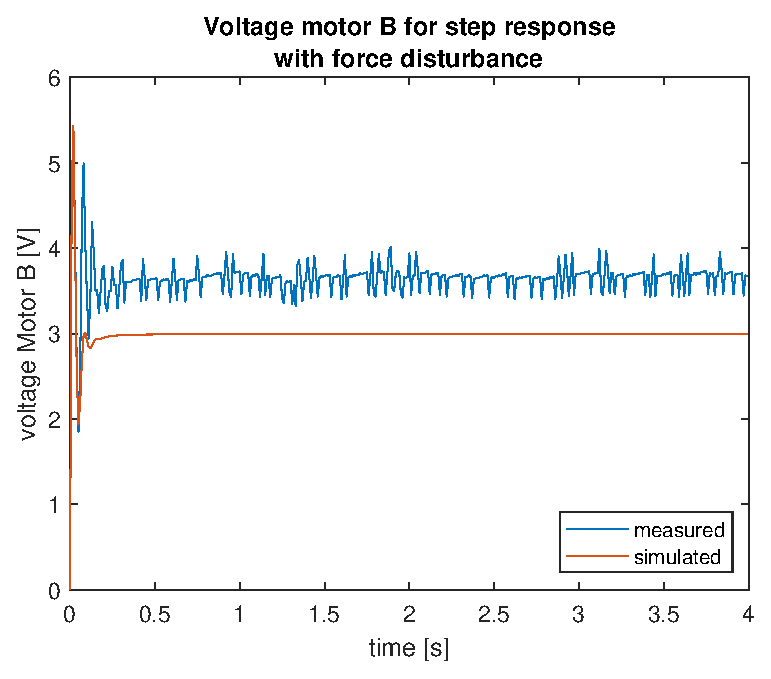
\includegraphics[width=\linewidth]{comparison_voltage_stepresponseB_FD.eps}
		
	\end{subfigure}
	\caption{Measured and simulated voltages for a step reference input with a constant force disturbance}
	\label{fig:voltagestepresponseFD}
\end{figure*}

In this section, the cart was placed on a slope to create a constant force disturbance. Other possibilities to achieve the same result are for example adding a weight to the cart itself, or letting the cart drag an additional weight. Both cases increase the drag force, between the wheels and the ground or between the extra weight and the ground respectively. Using the coulomb friction model, this increase in the drag force causes a constant friction force disturbance. Following the same reasoning as for the cart on a slope, the steady-state error will be zero as well. 

There are however also disturbances possible that do affect the steady-state tracking error. For example, if the cart is placed on a hill with an increasing slope, the force disturbance won't be constant and the steady-state error will not equal zero. At last, undulations of the road may cause a non-constant disturbance, which will affect the steady-state tracking error. 


\bibliographystyle{plain}
\bibliography{bibliography}

\end{document}